\chapter{Preliminary study}

In this chapter, we will conduct a preliminary study to establish a strong foundation for our project. This study will address critical areas necessary for understanding and planning the project efficiently. We will start with the basic concepts to ensure a solid grasp of the principles relevant to our work. Following this, we will perform a detailed requirements analysis, covering the initial setup, functional requirements, and non-functional requirements. We will utilize use case diagrams to illustrate system interactions and functionalities.

Additionally, we will present mockups to visualize the user interface, outline the product backlog to prioritize features and tasks, and explore the logical and physical architecture to detail the system structure.

Finally, we will review the technologies and tools to be used throughout the project. This comprehensive preliminary study will provide a robust framework for the design and implementation phases, ensuring all aspects of the project are well-planned and effectively executed.

\pagebreak

\section{Basic concepts}

\section{Cloud}
Cloud computing refers to an Internet-driven approach that delivers shared computing resources and data services to various devices as required. It is designed to provide ubiquitous, on-demand access to a collection of configurable computing resources (including networks, servers, storage, applications, and services) that can be quickly allocated and deallocated with minimal management effort. These cloud services offer both individuals and businesses the ability to store and manage data in data centers that are either privately operated or owned by third parties, which could be situated locally or internationally. The concept of cloud computing depends on resource sharing to maintain consistency and cost efficiency, akin to the operation of utilities such as the electrical grid.


\section{SaaS}
Software as a Service (SaaS) is a cloud computing model where software applications are hosted by a third-party provider and made available to customers over the internet. Users can access these applications via a web browser, eliminating the need to install or maintain software locally on their devices. This model offers convenience, scalability, and cost-effectiveness for both individual users and organizations.

\section{Software provisioning}
Software provisioning refers to the process of preparing and equipping a computer system with necessary software applications and configurations to fulfill specific operational requirements. It involves tasks such as installation, configuration, and initial setup of software components needed to support business operations or user requirements within an IT environment.


\section{Scalability}
Scalability refers to the capability of a system, network,
or process to handle a growing amount of work or its potential to be enlarged
to accommodate that growth. It is an essential characteristic for systems that are expected to expand over time.
Scalability can be vertical or horizontal:

$\bullet$ \textbf{Vertical Scalability (Scaling Up)}: This involves adding more power (such as CPU, RAM) to an existing machine. It means enhancing the capacity of a single resource.

$\bullet$ \textbf{Horizontal Scalability (Scaling Out)}: This involves adding more machines or devices to a system so that the workload and processing power are distributed across multiple units.

In the context of computing and business applications, scalability ensures that the system can maintain or improve its performance and efficiency as the demand for resources or services increases. It is a critical factor in the design and architecture of applications, especially those that require handling large volumes of data or high user traffic.

\section{ Containerization}
Containerization is a lightweight form of virtualization that involves
encapsulating an application and its dependencies into a container. 
This container is a standardized unit of software that packages up the code and all its dependencies so the application runs quickly and reliably from one computing environment to another.

\section{Serverless computing}
Serverless computing, also referred to as Function as a Service (FaaS), is a cloud computing model in which the cloud provider takes care of the infrastructure required to run code. This allows developers to concentrate on creating and deploying specific functions or segments of business logic without the need to manage servers or hardware.


\section{REST architecture}
REST, which stands for Representational State Transfer, is an architectural style used for designing networked applications. It facilitates the creation and modification of resources with ease, serving as a lightweight alternative to complex mechanisms such as RPC, CORBA, and SOAP.

REST is not a formal standard but a set of guidelines for building efficient communication frameworks between two machines using the HTTP protocol. The World Wide Web, which operates over HTTP, can be seen as a prime example of a REST-based architecture. REST utilizes a stateless, client-server, cacheable communication protocol, making it simple to implement and maintain. Furthermore, it enhances scalability by supporting multiple backend services simultaneously.

Similar to web services, a REST service is platform-independent and language-independent, operating over HTTP and functioning effectively even behind firewalls.

There are several fundamental concepts that distinguish REST from other web services. These key principles include:

$\bullet$ \textbf{Unique URL-Resource mapping}: Each resource is associated with a unique URL, providing a logical way to access specific information. 

$\bullet$ \textbf{Statelessness}: All information required to process a request is included within the request itself, meaning the server does not retain any state from previous requests. This principle is derived from the stateless nature of HTTP.

$\bullet$ \textbf{Action Verbs}: REST uses HTTP verbs to specify the action to be performed. The primary HTTP verbs in REST architecture are GET, POST, PUT, and DELETE. GET retrieves resources, PUT updates resources, POST creates new resources, and DELETE removes resources.

$\bullet$ \textbf{Data Exchange formats}: REST does not mandate a specific data encoding format for resource bodies. Common formats include JSON \cite{json} and XML, but others like PROTOBUF and YAML are also supported.


% \subsection{Numeric Metrics}
% \begin{itemize}
%     \item \textbf{Accuracy}: We report class-wise accuracy by considering True Positive (TP) as the positive reviews which were
% correctly predicted as positive, and True Negative (TN) as those reviews which were correctly classi-
% fied as negative. Then, False Positives (FP) and False Negatives (FN) follow intuitively. The actual
% accuracy of the models were obtained with Equation \ref{eq1}.

% \begin{equation} \label{eq1}
% Accuracy = \frac{TP+TN}{TP+FP+TN+FN}
% \end{equation}
%     \item \textbf{True Positive Rate/Recall/Hit Rate/Sensitivity}: The true positive rate (TPR) measures the proportion of correctly identified actual positives (TP).

% \begin{equation} \label{eq1}
% TPR = \frac{TP}{TP+FN} = 1 - False Negative Rate
% \end{equation}
% \item \textbf{ False Positive Rate/Fall-Out } : The false positive rate (FPR) measures the proportion of incorrectly identified actual negatives (FP).
% \begin{equation} \label{eq1}
% FPR = \frac{FP}{FP+TN} = 1 - Specificity
% \end{equation}

% \end{itemize}



% \subsection{Vendor lock-in}
\section{Vendor lock-in}

Vendor lock-in is a situation where a customer becomes dependent on a specific vendor for products and services,
making it difficult to switch to another provider without incurring significant costs, inconvenience,
or compatibility issues. This dependency can arise from various factors such as proprietary technologies,
unique data formats, or specific software that are incompatible with other vendors' systems.
Vendor lock-in can lead to reduced flexibility, higher costs, and increased risk for the customer,
as they may struggle to adapt to new technologies or negotiate better terms. To mitigate vendor lock-in, organizations can adopt open standards, ensure data portability, negotiate flexible contracts, and diversify their technology stack across multiple vendors.


\section{Orchestration}
Orchestration in computing refers to the automated arrangement, coordination, and management of complex computer systems, middleware, and services. It involves organizing multiple automated tasks and workflows to ensure they function together seamlessly, often in cloud environments, containers, and microservices architectures. Orchestration tools streamline and simplify the deployment, scaling, and operations of applications, enabling efficient resource use, consistency, and scalability.




\section{Requirements analysis}

%\subsection{Design session}
%After  the beginning of the internship, we had a on-month training where we were
%trained about the different technologies that Pulpetech is using, such as Django, Angular, PostgreSQL.. %technologies
%Also, as interns, we had the opportunity, first, to get
%familiar with the company's working environment, second, understand better the
%project's goal and its added value to its users, and third, were able to collect
%the functional and non functional requirements of the project.
\subsection{Functional Requirements}
The overall goal of this project is to develop a comprehensive dashboard for real-time management and monitoring of cloud resources, specifically tailored to support the operational needs of Ilef. The platform is designed exclusively for use by Cloud/DevOps engineers, providing detailed control and oversight of various cloud environments. The following functionalities are essential:

\subsubsection{Initial Setup and Configuration}
Before utilizing the main features of the dashboard, the following servers must be deployed and configured:
\begin{itemize}
    \item \textbf{Jira}: For project management.
    \item \textbf{Mattermost}: For team communication.
    \item \textbf{Glitchtip}: For error and performance monitoring.
    \item \textbf{Jenkins}: For automating builds and deployment pipelines.
    \item \textbf{Vault}: For managing and securing secrets.
    \item \textbf{Nexus}: For storing and managing Docker images and other artifacts.
    \item \textbf{SonarQube}: For continuous inspection of code quality.
\end{itemize}

\subsubsection{Core Functionalities}
The dashboard provides several critical functionalities for the Cloud/DevOps engineer:
\begin{itemize}
    \item \textbf{Authentication}: Ensure secure access to the platform, allowing only authorized Cloud/DevOps engineers to log in and interact with the system.
    \item \textbf{Virtual Machine Management}: Enable the manual provisioning, configuration, and management of virtual machines across multiple cloud providers, including AWS, Azure, GCP, and Hetzner. This includes starting, stopping, restarting, and deleting virtual machines.
    \item \textbf{Bucket Management}: Allow engineers to manually upload, retrieve, and delete objects within storage buckets across AWS, Azure, and GCP, providing flexible data management options.
    \item \textbf{Docker Image Management}: Facilitate the uploading of Docker images directly to virtual machines and support the creation of Kubernetes clusters from these images for container orchestration.
    \item \textbf{Nexus Repository Operations}: Enable easy retrieval of Docker images stored in the Nexus repository, facilitating efficient image management and deployment.
    \item \textbf{Vault Secret Management}: Provide secure access to and management of secrets stored in the Vault server, essential for the configuration and operation of applications and infrastructure.
    \item \textbf{Scrumboard Management}: Integrate a Scrumboard within the platform that allows Cloud/DevOps engineers to create, update, and track tasks throughout the development cycles, enhancing organizational capabilities and project tracking.
\end{itemize}

\subsubsection{Building Advanced Visualization Tools}
To support effective resource management, the platform includes advanced visualization tools:
\begin{itemize}
    \item \textbf{Interactive Data Visualization}: Develop a dashboard that provides interactive charts and graphs detailing current resource usage, historical data, and predictive analytics, enabling users to interact with the data and gain new insights.
    \item \textbf{Customizable Data Views}: Allow users to customize views and filters to display data based on various parameters such as resource type, usage statistics, and provider, enhancing their ability to monitor and manage resources effectively.
\end{itemize}

\subsection{Non-Functional Requirements}

\subsubsection{Performance}
\begin{itemize}
    \item \textbf{Efficiency}: The platform should manage operations like virtual machine administration, bucket handling, and Docker image processing swiftly and with minimal latency.
    \item \textbf{Response Time}: Tasks such as starting or stopping a virtual machine should complete within a few seconds.
    \item \textbf{Throughput}: The system needs to handle multiple simultaneous operations efficiently, ensuring high throughput and minimizing user wait times.
    \item \textbf{Scalability}: The platform must scale effectively to manage increased loads, allowing numerous users to perform tasks concurrently without significant performance loss.
\end{itemize}

\subsubsection{Reliability}
\begin{itemize}
    \item \textbf{System Stability}: The platform should deliver consistent performance and maintain high reliability with minimal downtime.
    \item \textbf{Maintenance}: Conduct maintenance during off-peak hours and notify users in advance to minimize disruptions.
    \item \textbf{Monitoring and Alerts}: Establish thorough monitoring and alerting mechanisms to quickly identify and resolve issues, ensuring continuous operation and minimal downtime.
    \item \textbf{Data Integrity}: Maintain data integrity by detecting and preventing unauthorized modifications.
\end{itemize}

\subsubsection{Maintainability}
\begin{itemize}
    \item \textbf{Modular Architecture}: Develop the system using a modular architecture to facilitate easy updates, maintenance, and scalability.
    \item \textbf{Logging and Monitoring}: Implement detailed logging and monitoring systems to promptly identify and address issues, ensuring the platform's overall health and performance.
\end{itemize}


\section{Requirement specifications}
\subsection{Actors Identification}

The Ilef management platform is designed for Cloud/DevOps engineers and administrators, each with distinct roles and responsibilities within the system.

\subsubsection{User Roles}

\paragraph{Cloud/DevOps Engineer}
\begin{itemize}
    \item \textbf{Role Description}: This user primarily engages with the platform to oversee and manage cloud resources and will be referred to as \textbf{"User"} throughout the rest of the report.
    \item \textbf{Key Functions}:
    \begin{itemize}
        \item Log in and authenticate
        \item Administer virtual machines on AWS, Azure, GCP, and Hetzner
        \item Manage objects in cloud storage buckets on AWS, Azure, and GCP (upload, fetch, delete)
        \item Deploy Docker images to virtual machines
        \item Set up Kubernetes clusters from Docker images
        \item Retrieve Docker images from the Nexus repository
        \item Access secrets stored in the Vault server
        \item Use the Scrumboard for task management
    \end{itemize}
\end{itemize}

\paragraph{Administrator}
\begin{itemize}
    \item \textbf{Role Description}: This user has comprehensive access to all platform features, including advanced user management functions.
    \item \textbf{Key Functions}:
    \begin{itemize}
        \item Perform all functions available to Cloud/DevOps Engineers
        \item Create, modify, and delete user accounts
    \end{itemize}
\end{itemize}


\subsection{Use cases diagrams}
\begin{itemize}

    \item The following figure  \hyperref[fig:general_use_cases]{\ref{fig:general_use_cases}} introduces the general use cases which present the
functionalities of the application.

\begin{figure}[htbp]
  \center
  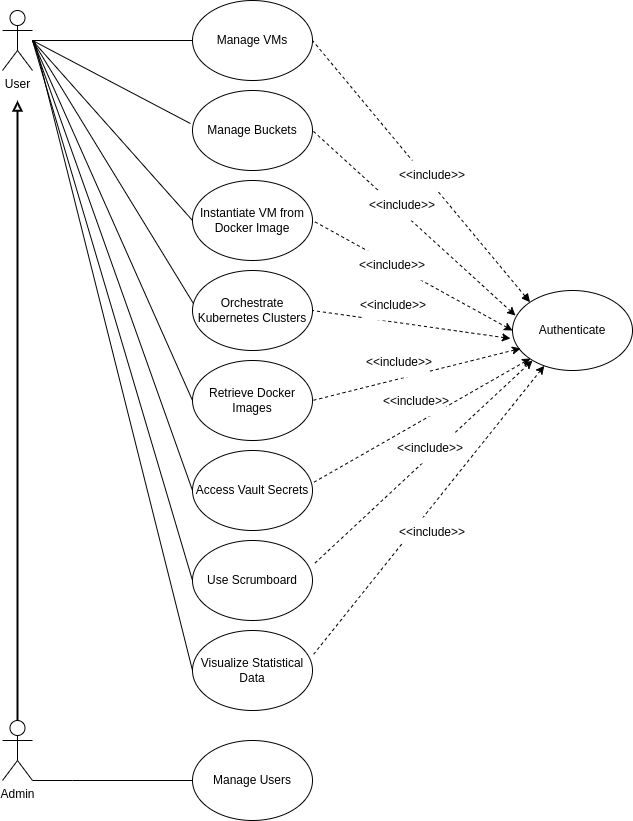
\includegraphics[width=19cm]{general_use_cases}
  \caption{General use case diagram}
  \label{fig:general_use_cases}
\end{figure}




\end{itemize}


\section{Mockups}
In this section, we will outline and confirm the business requirements for the project by presenting UI views 
with the help of mockups. We will begin by introducing the Penpot tool,
followed by a detailed explanation of the project's mockups.



\subsection{Penpot}
We suggested using Penpot, an open-source graphical tool for designing user interfaces for websites and
web/desktop/mobile applications. Mockups created with Penpot provide enough interactivity to replace prototypes,
making it easy to collaborate and get feedback on the wireframes. It is defined on their website as \href{https://penpot.app/}{\textit{"Penpot is the web-based open-source design tool that bridges the gap between designers and developers."}}


\subsection{Project mockups}
In this section, we will describe the mockups for our project’s components.

UI General Description:
The dashboard consists of six main screens: main dashboard statistics, instances, storages, vault secrets, clusters, and Docker screens. Below, we will describe the mockups and the requirements for each view.

\subsubsection{Dashboard statistics page}

The figure \hyperref[fig:mockup-dashboard]{\ref{fig:mockup-dashboard}} represents the landing page of our application.
\begin{figure}[h]
  \center
  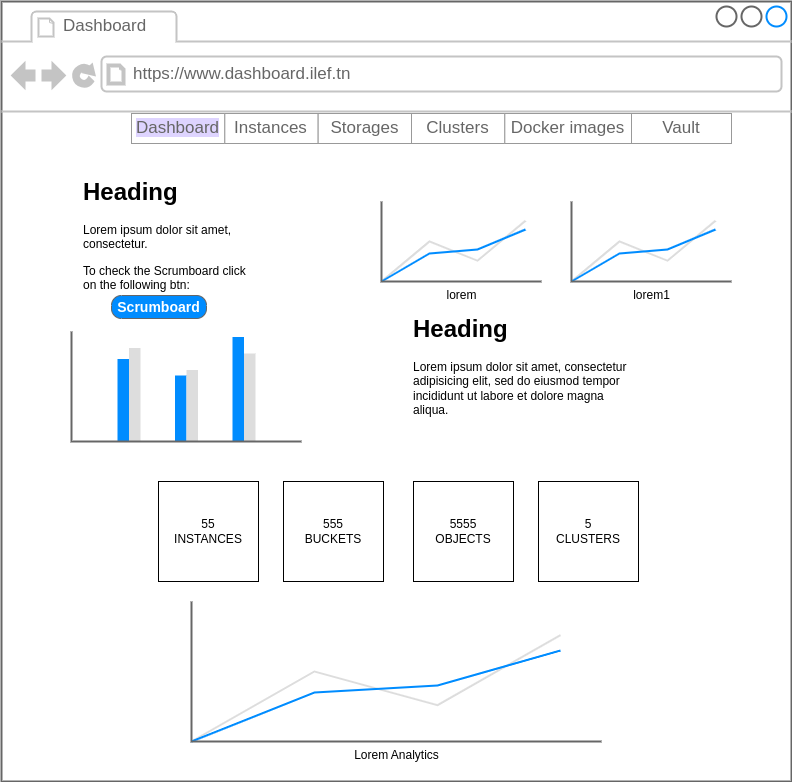
\includegraphics[width=13cm]{mockup-dashboard.png}
  \caption{Main dashboard page mockup}
  \label{fig:mockup-dashboard}
\end{figure}
\vspace{50mm}

\subsubsection{Instances page}

The mockup \hyperref[fig:mockup-instances]{\ref{fig:mockup-instances}} represents the page of instances of our application, featuring buttons for adding, stopping, rebooting, and terminating instances.

\begin{figure}[h]
  \center
  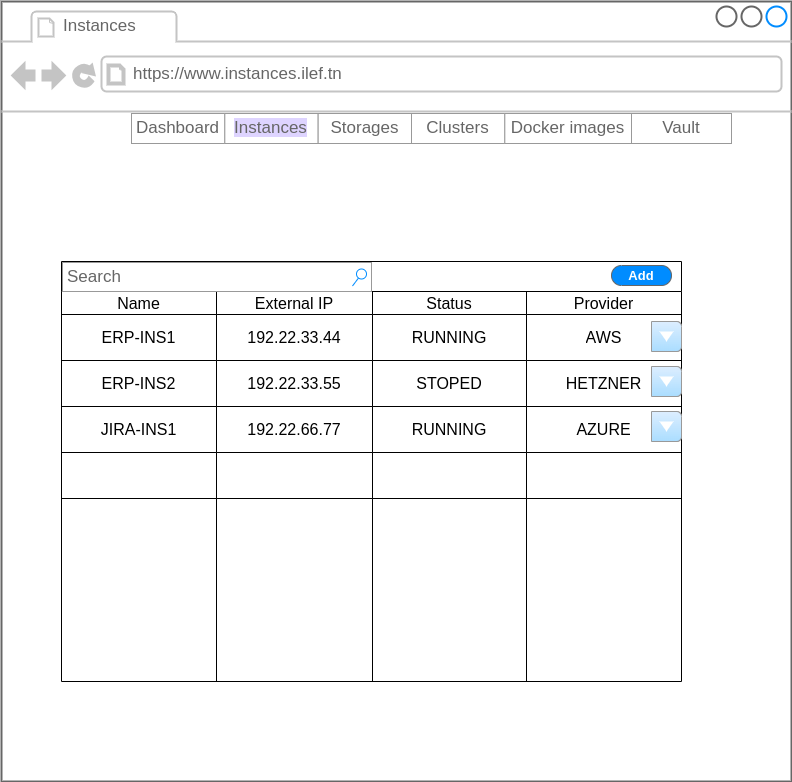
\includegraphics[width=13cm]{mockup-instances.png}
  \caption{Instance page mockup}
  \label{fig:mockup-instances}
\end{figure}
% \vspace{50mm}

\subsubsection{Storages page}

The mockup \hyperref[fig:mockup-storages]{\ref{fig:mockup-storages}} depicts the storage page of our application, with buttons for uploading, deleting, and generating presigned URLs.

\begin{figure}[h]
  \center
  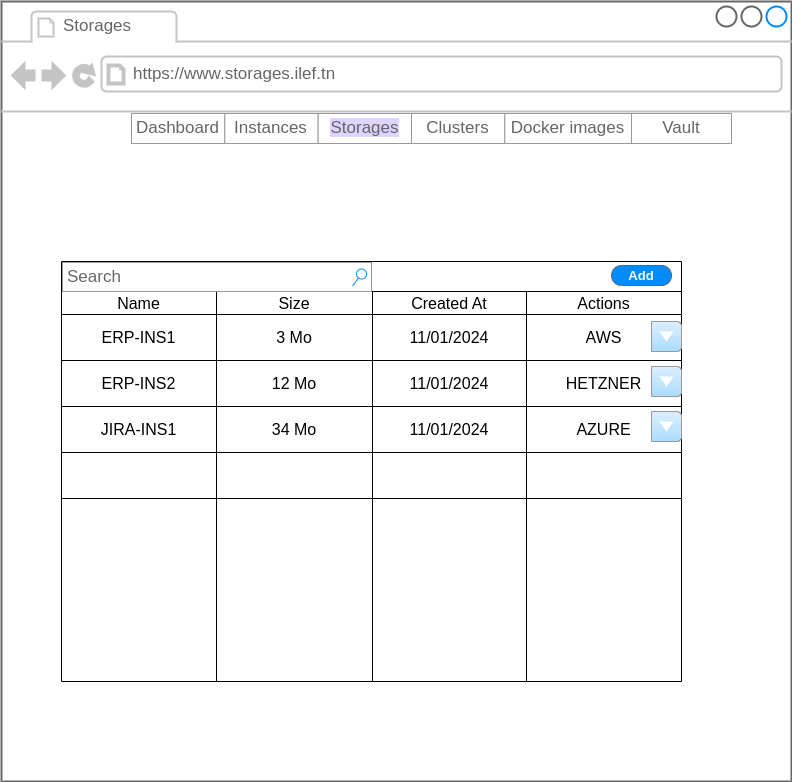
\includegraphics[width=13cm]{./chapters/preliminary_study/mockup-storages.png}
  \caption{Storages page mockup}
  \label{fig:mockup-storages}
\end{figure}

\vspace*{3cm}
\subsubsection{Docker images page}


The mockup \hyperref[fig:mockup-images]{\ref{fig:mockup-images}} represents the page of Ilef images of our application with buttons to instantiate to a server for different cloud providers.

\begin{figure}[h]
  \center
  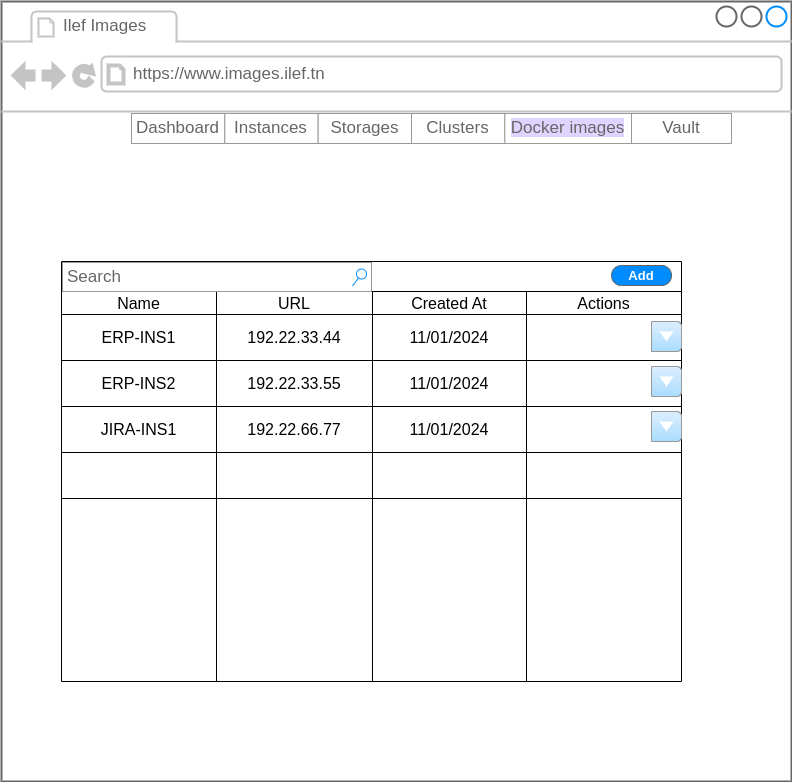
\includegraphics[width=13cm]{./chapters/preliminary_study/mockup-images.png}
  \caption{Ilef images page mockup}
  \label{fig:mockup-images}
\end{figure}

\vspace*{2cm}

\subsubsection{Vault secrets page}

The mockup \hyperref[fig:mockup-vault]{\ref{fig:mockup-vault}} represents the Ilef vault page of our application, fetching data from the Nexus server, with buttons to add, delete, and update.

\begin{figure}[h]
  \center
  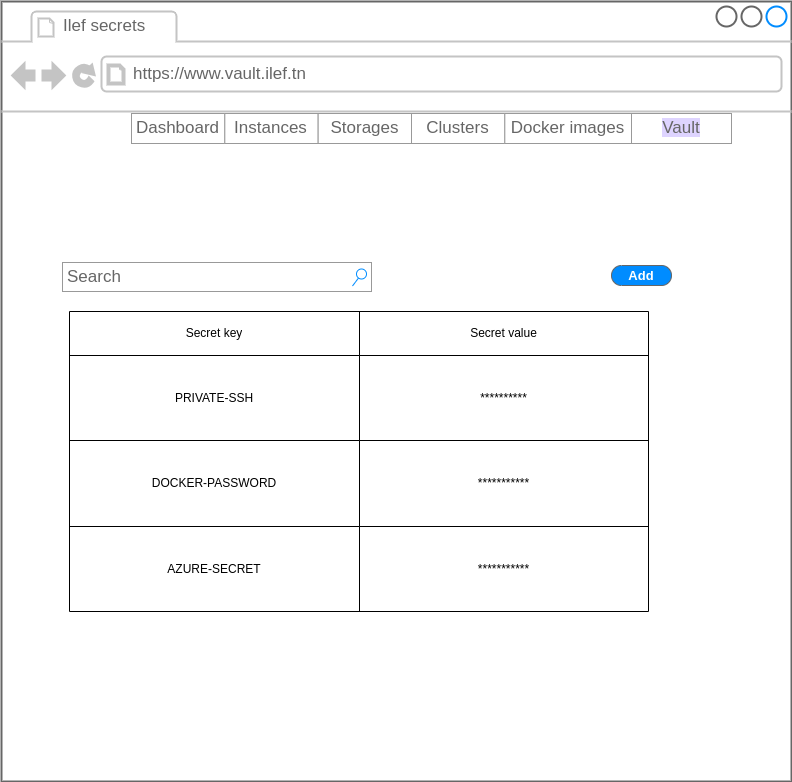
\includegraphics[width=13cm]{./chapters/preliminary_study/mockup-vault.png}
  \caption{Ilef vault page mockup}
  \label{fig:mockup-vault}
\end{figure}

\subsubsection{Cluster page}


The mockup \hyperref[fig:mockup-clusters]{\ref{fig:mockup-clusters}} represents the Ilef cluster page of our application, with buttons to add, delete, drain, and uncordon nodes.

\begin{figure}[h]
  \center
  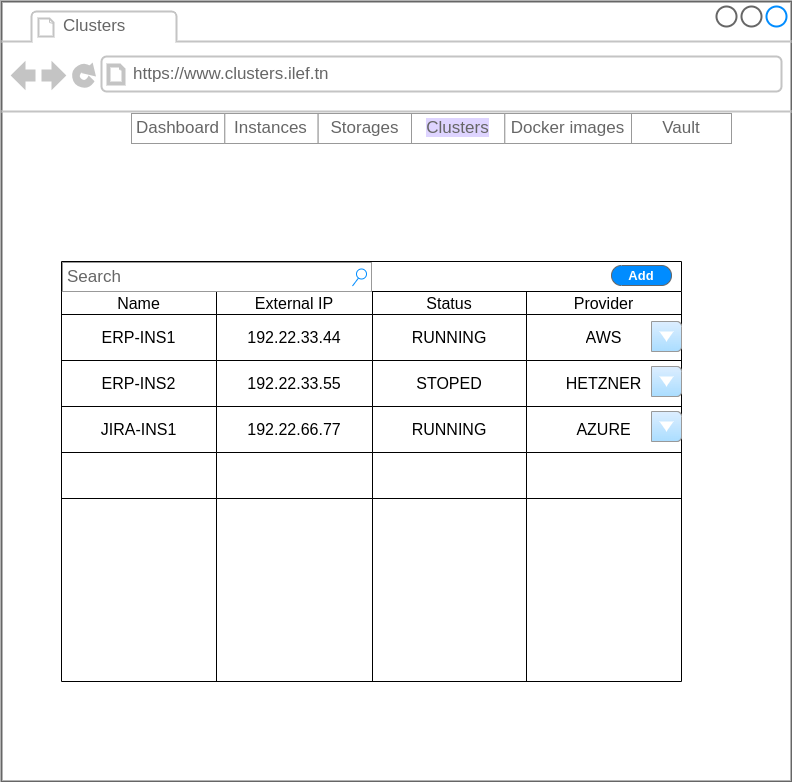
\includegraphics[width=13cm]{./chapters/preliminary_study/mockup-clusters.png}
  \caption{Ilef clusters page mockup}
  \label{fig:mockup-clusters}
\end{figure}

\vspace*{3cm}
\section{Product Backlog}

Based on the previous requirements, we derived the product backlog described in Table \ref{tab:product_backlog}.

After the product backlog was established and validated by the Product Owner, the scrum team divided it into five sprints. The sprint durations were suggested by the Scrum Master, with each sprint planned to last one month as shown in Table \ref{tab:sprints_backlog}.

\begin{longtable}{|p{1cm}|p{8cm}|p{2cm}|p{2cm}|}
  \caption{Product Backlogs of Ilef Project} \label{tab:product_backlog} \\
  \hline
  \textbf{ID} & \textbf{User Story} & \textbf{Priority} & \textbf{Estimation (days)} \\
  \hline
  \endfirsthead
  \multicolumn{4}{c}%
  {\tablename\ \thetable\ -- \textit{Continued from previous page}} \\
  \hline
  \textbf{ID} & \textbf{User Story} & \textbf{Priority} & \textbf{Estimation (days)} \\
  \hline
  \endhead
  \hline \multicolumn{4}{r}{\textit{Continued on next page}} \\
  \endfoot
  \hline
  \endlastfoot
  
  1 & As a user, I can log in to the platform securely to access my dashboard and functionalities. & High & 8 \\
  \hline
  2 & As a user, I can view various charts and bar graphs that display statistics and metrics relevant to my cloud resources. & Medium & 10 \\
  \hline
  3 & As a user, I can easily manage instances (create, start, stop, restart, and delete) across different cloud providers (AWS, Azure, GCP, Hetzner). & High & 10 \\
  \hline
  4 & As a user, I can manage storage solutions, including uploading, fetching, and deleting objects, across different cloud providers (AWS, Azure, GCP). & High & 10 \\
  \hline
  5 & As a user, I can quickly deploy a Docker image to a virtual machine instance. & Medium & 6 \\
  \hline
  6 & As a user, I can create a Kubernetes cluster from a Docker image for container orchestration. & Medium & 15 \\
  \hline
  7 & As a user, I can manage and retrieve secrets from the vault server securely. & High & 8 \\
  \hline
  8 & As a user, I can fetch Docker images stored in the Nexus repository for deployment. & Medium & 6 \\
  \hline
  9 & As a user, I can use the integrated Scrumboard to manage and track project tasks and progress. & Medium & 10 \\
  \hline
  10 & As an admin, I can manage user accounts, including creating, modifying, and deleting accounts, and assigning roles and permissions. & High & 4 \\
  \hline
  11 & As a developer, I can set up a CI/CD pipeline to automate the build, test, and deployment processes for the project. & High & 20\\
  \hline
  \end{longtable}

\begin{table}[h!]
\centering
\caption{User Stories through each sprint}
\label{tab:sprints_backlog}
\begin{tabular}{|p{2cm}|p{10cm}|p{2cm}|}
\hline
\textbf{Sprint} & \textbf{User Stories} & \textbf{Estimation (days)} \\ \hline
Sprint 1 
& As an admin, I can manage user accounts, including creating, modifying, and deleting accounts, and assigning roles and permissions. & 4 \\ \cline{2-3}
& As a user, I can log in to the platform securely to access my dashboard and functionalities. & 8 \\ \cline{2-3}
& As a user, I can manage and retrieve secrets from the vault server securely. & 8  \\ \hline

\multirow{2}{*}{Sprint 2} 
& As a user, I can easily manage instances (create, start, stop, restart, and delete) across different cloud providers (AWS, Azure, GCP, Hetzner). & 10 \\ \cline{2-3}
& As a user, I can manage storage solutions, including uploading, fetching, and deleting objects, across different cloud providers (AWS, Azure, GCP). & 10 \\ \hline

\multirow{3}{*}{Sprint 3}
& As a user, I can quickly deploy a Docker image to a virtual machine instance. & 6 \\ \cline{2-3}
& As a user, I can create a Kubernetes cluster from a Docker image for container orchestration. & 8 \\ \cline{2-3}
& As a user, I can fetch Docker images stored in the Nexus repository for deployment. & 6 \\ \hline

\multirow{2}{*}{Sprint 4}
& As a user, I can use the integrated Scrumboard to manage and track project tasks and progress. & 10 \\ \cline{2-3}
& As a user, I can view various charts and bar graphs that display statistics and metrics relevant to my cloud resources. & 10  \\ \hline
\multirow{1}{*}{Sprint 5}
& As a developer, I can set up a CI/CD pipeline to automate the build, test, and deployment processes for the project. & 20  \\ \hline
\end{tabular}
\end{table}

\section{Sprint Planning}
Our work will be divided into 4 sprints as follows, with each sprint focusing on the design and development of several modules:
\begin{itemize}
  \item \textbf{Sprint 1: User management}
  \item \textbf{Sprint 2: Computing and Storages management}
  \item \textbf{Sprint 3: Container management}
  \item \textbf{Sprint 4: Data visualization and projects management}
  \item \textbf{Sprint 5: Implementing CI/CD}
\end{itemize}


\section{Logical and Physical Architecture}

Our physical architecture application is based on a three-tier architecture as shown in \hyperref[fig:archi-phy]{Figure: (\ref{fig:archi-phy})}, also known as a three-layer architecture, which follows a client-server model.
\begin{itemize}
  \item \textbf{Persistent Data Access Layer:}  This first layer involves a server that hosts the database, managing the storage and retrieval of persistent data.
  \item \textbf{Business Logic Processing Layer:}  The second layer includes a web server that handles client requests and a client server responsible for business logic and processing.
  \item \textbf{Data Presentation Layer:}   The third layer is the application itself, presenting data to the user and managing user interactions.
\end{itemize}

\begin{figure}[h]
  \center
  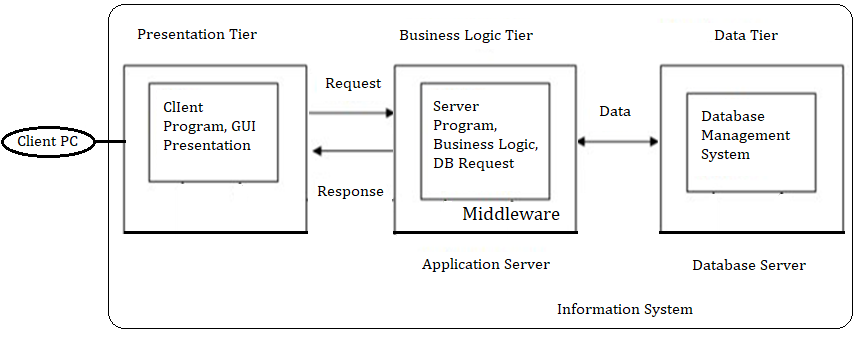
\includegraphics[width=17cm]{./chapters/preliminary_study/archi-phy.png}
  \caption{Physical architecture of Ilef application}
  \label{fig:archi-phy}
\end{figure}


The following figure {Figure: (\ref{fig:archi-log})} represents the logical architecture of our application and outlines the interaction between different components.
\vspace*{3cm}

\begin{figure}[h]
  \center
  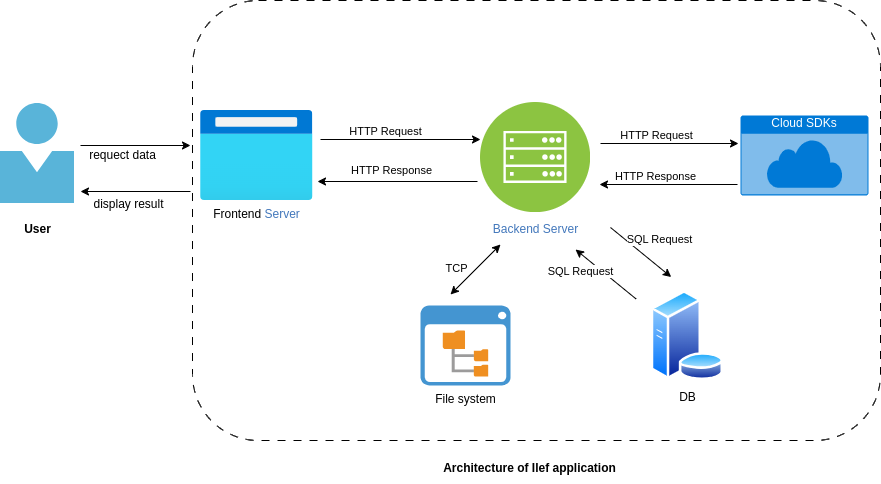
\includegraphics[width=15cm]{./chapters/preliminary_study/archi-logique.png}
  \caption{Logical architecture of Ilef application}
  \label{fig:archi-log}
\end{figure}

\section{Used technologies}

\subsection{Programming languages}
In this section, we give an overview on the programming languages used to implement our solution.
\subsubsection{Python}
Python is an interpreted, interactive, object-oriented programming language. It incorporates modules, exceptions, dynamic typing, high-level dynamic data types, and classes. Python combines significant power with clear syntax. It has interfaces to many system calls and libraries, as well as to various window systems, and is extensible in C or C++. It is also usable as an extension language for applications requiring a programmable interface. Finally, Python is portable: it runs on many Unix variants, Mac, and PCs under MS-DOS, Windows, Windows NT, and OS/2.

Python is a high-level, general-purpose programming language applicable to many problem domains. It comes with a large standard library covering areas such as string processing (regular expressions, Unicode, file differences), Internet protocols (HTTP, FTP, SMTP, XML-RPC, POP, IMAP, CGI programming), software engineering (unit testing, logging, profiling, parsing Python code), and operating system interfaces (system calls, filesystem, TCP/IP sockets). The Python Standard Library's table of contents provides an overview of its capabilities. Additionally, a wide variety of third-party extensions are available.\cite{python}

\subsubsection{TypeScript}
TypeScript is an open-source programming language developed and maintained by Microsoft. It is a strict syntactical superset of JavaScript that adds optional static typing. TypeScript is designed for developing large applications and transcompiles to JavaScript. As a superset of JavaScript, existing JavaScript programs are valid TypeScript programs.\cite{typescript}

\subsection{Frameworks}
\subsubsection{Angular}

Angular is an open-source front-end framework developed by Google for creating dynamic, modern web applications. First introduced in 2009, the framework has gained significant traction over the years for reducing unnecessary code and ensuring lighter, faster applications. Rapidly evolving from AngularJS in 2010 to Angular 9 in 2020, it is now used by more than 25.1% of software engineers for creating user interfaces (Stack Overflow Developer Survey 2020 \cite{angular}). Angular facilitates the development of interactive and dynamic single-page applications (SPAs) with features such as templating, two-way binding, modularization, RESTful API handling, dependency injection, and AJAX handling. Designers can use HTML as a template language and extend HTML syntax to easily define application components.

\subsubsection{Django}
Django is a high-level Python web framework designed for the rapid development of secure and maintainable websites. Created by experienced developers, Django alleviates much of the complexity of web development, allowing you to focus on building your application without reinventing the wheel. It is free, open-source, and supported by a vibrant, active community. Additionally, Django offers excellent documentation and numerous options for both free and paid support \cite{django}.


\subsection{Cloud services and tools}
\subsubsection{AWS}
Amazon Web Services (AWS) is a comprehensive cloud computing platform provided by Amazon, offering a variety of services such as computing power, storage options, and networking capabilities. AWS enables businesses to build, deploy, and manage applications and services efficiently.

\subsubsection{Google Cloud platform}
Google Cloud Platform (GCP) is a suite of cloud computing services provided by Google that runs on the same infrastructure used for its end-user products. GCP offers a range of services, including computing, storage, data analytics, and machine learning.

\subsubsection{Microsoft Azure}
Microsoft Azure is a cloud computing service created by Microsoft for building, testing, deploying, and managing applications and services through Microsoft-managed data centers. It provides software as a service (SaaS), platform as a service (PaaS), and infrastructure as a service (IaaS).

\subsubsection{Hetzner}
Hetzner Online is a professional web hosting service provider and experienced data center operator in Germany. It offers scalable virtual machines and cloud instances through Hetzner Cloud, high-performance storage solutions with Hetzner Storage Box, and load balancing with Hetzner Load Balancer. Hetzner's services are known for their reliability and cost-effectiveness.

\subsubsection{Jenkins}
Jenkins is an open-source automation server that helps automate software development tasks related to building, testing, and deploying, facilitating continuous integration and continuous delivery (CI/CD). Jenkins supports a wide range of plugins to extend its functionality and integrate with other tools. Maintained by a community of developers, Jenkins is widely used in DevOps practices.

\subsubsection{Ansible}
Ansible is an open-source software provisioning, configuration management, and application deployment tool that enables infrastructure as code. It automates cloud provisioning, configuration management, application deployment, and various other IT tasks. Ansible uses a simple language (YAML) to describe automation jobs and can manage thousands of servers simultaneously. Ansible is developed by Red Hat.

\subsubsection{Glitchtip}
Glitchtip is an open-source error and performance monitoring tool that helps developers track and fix bugs in real-time. It provides comprehensive reports and integrates with various development environments, enabling teams to monitor application performance and manage errors efficiently. Glitchtip is maintained by a community of developers.

\subsubsection{HashiCorp Vault}
HashiCorp Vault is a tool for securely accessing secrets, such as API keys, passwords, certificates, and other sensitive data. It provides a unified interface to manage secrets, implements tight access control, and maintains a detailed audit log of all accesses. Vault integrates with various authentication methods and is highly scalable, making it suitable for both small and large organizations.

\subsubsection{Nexus Repository}
Nexus Repository is a repository manager for storing and managing development artifacts, including binaries, build artifacts, and Docker images. It helps teams store and retrieve components efficiently, ensuring that the correct version of an artifact is used in builds and deployments. Nexus Repository supports various repository formats, including Maven, npm, NuGet, and Docker. Nexus Repository is developed by Sonatype.

\subsubsection{SonarQube}
SonarQube is an open-source platform for continuous inspection of code quality, performing automatic reviews with static analysis to detect bugs, code smells, and security vulnerabilities. It provides detailed reports and integrates with various development tools and CI/CD pipelines. SonarQube supports multiple programming languages and helps ensure that code quality and security standards are maintained. SonarQube is developed by SonarSource.


\section*{Conclusion}
In this chapter, we have conducted a comprehensive preliminary study to establish a solid foundation for our project. This study covered essential areas, including basic concepts and a detailed requirements analysis. We specified requirements through use case diagrams and provided mockups to visualize the user interface. Additionally, we outlined the product backlog to prioritize features and tasks and explored the logical and physical architecture to detail the system structure. We also reviewed the technologies and tools to be utilized throughout the project.

This thorough preliminary study has equipped us with a clear understanding and strategic plan for the project's design and implementation phases. By addressing all critical aspects early on, we have ensured that the project is well-prepared for successful execution and delivery.